\chapter{Statistik und Leistungsmessung}
\section{Einleitung}
\begin{table}[h]
	\centering
	\begin{tabular}{|c|c|}
		\hline 
		Teilübung 	& Statistik und Leistungsmessung \\
		\hline 
		Teilübungsnr. 		& 2	 \\ 
		\hline 
		Datum 		& 28.11.2018 \\ 
		\hline 
		Messplatzbez. 	& CA \\
		\hline
	\end{tabular} 
	\caption{Grundlegende Information der 2. Laborübung}
\end{table}
\noindent
Im Rahmen der 2. Laborübung sollten fünf unterschiedliche Impedanzen ($Z1$ - $Z5$) vermessen werden. Dabei war lediglich deren Struktur (siehe Tabelle \ref{tb:imp}!) im Vorhinein bekannt. Es wurde zuerst ein passender Strommessshunt ausgewählt und die Schaltung konzipiert. Um aus den erhaltenen Spannungswerten den dazugehörigen Strom bestimmen zu können ist natürlich die genau Kenntnis über den Widerstandswert unabdingbar, weshalb dieser zu Beginn mehrmals und mit unterschiedlichen Methoden bestimmt worden ist. Die eigentliche Impedanzmessung wurde darauf hin mit einem analogen Oszilloskop durchgeführt. \\
Alle dabei verwendenten Messgeräte sind in Tabelle \ref{tb:messgeraete} aufgelistet.
\begin{table}[h]
	\begin{tabular}{|c|c|}
	\hline 
	Gerät & Bezeichnung \\ 
	\hline 
	Handmultimeter & Agilent U1232A \\ 
	\hline 
	Handmultimeter & Mastech MS8221C \\ 
	\hline 
	Handmultimeter & Neumann 9140 \\ 
	\hline 
	Desktopmultimeter & Agilent 34461A \\ 
	\hline 
	Analoges Oszilloskop & XXXX-------XXX DS-6612 \\ 
	\hline 
	LCR-Meter & XXXX------- \\ 
	\hline 
	Digitales Speicheroszilloskop & XXXX------\\ 
	\hline 
	\end{tabular} 
	\centering
	\caption{Verwendete Messgeräte}
	\label{tb:messgeraete}
\end{table}

\subsubsection{Eigentumsbestätigung}
Hermit bestätigen die Studierenden der Gruppe 20, alle Messungen selbst durchgeführt und für die Berechnungen ausschließlich diese Messergebnisse herangezogen zu haben. \\ \\
\begin{tabular*}{\textwidth}{c|c|c}
	Patrick Mayr & Katharina Kralicek & Oskar Fürnhammer \\ 
	01526681 & 01611844 & 01329133 \\ 
\end{tabular*}


\section{Strommessung}
Um den Strom durch einen bestimmten Strang zu messen musste zuerst eine passende Schaltung entworfen bzw. in weiterer Folge ein passender Messshunt ausgewählt werden. Unter der Bedingung, dass bei einer Eingangsspannung von $U=10\,V_{\text{pp}}$ ein maximaler Strom von $I_{\text{max}}=5\,$mA nicht überschritten werden soll, ergibt sich mit dem Ohm'schen Gesetzt direkt
\begin{equation}
	R_{i,\text{min}} = \frac{\hat{U}}{I_{max}} = \frac{5\,\text{V}}{5\,\text{mA}} = 1\,\text{k}\Omega
	\label{eq:widerstandsdim}
\end{equation}
\section{Widerstandsmessung}
Da 
\begin{table}[h]
	\centering
	\begin{tabular}{|l|c|c|}
	\hline 
	Messung & Widerstandswert $R_i$ [$\Omega$]\\ 
	\hline 
	M1 - Agilent U1232A & 986		\\ 
	\hline 
	M2 - Mastech MS8221C & 984		\\ 
	\hline 
	M3 - Neumann 9140 & 988		\\ 
	\hline 
	DM - Agilent 34461A & 987		\\ 
	\hline 
	\end{tabular}
	\caption{Gemessene Widerstandswerte}
	\label{tb:widerstandswerte}
\end{table} \noindent
Damit ergibt sich der Mittelwert zu
\begin{equation}
	\overline{R_i} = \frac{1}{N} \sum\limits_{j=0}^N R_{i,j} = 986.25\, \Omega
	\label{eq:mittelw}
\end{equation}
Die empirische Standardabweichung wurde wiederum folgendermaßen berechnet:
\begin{equation}
	s(\overline{R_i}) = \sqrt{\frac{1}{N-1} \sum\limits_{j=0}^N (R_{i,j} - \overline{R_i})^2} = 1.7078\, \Omega 
	\label{eq:stdabw}
\end{equation}
Das Desktopmultimeter bietet die Funktion diverse statistische Größen direkt zu berechnen. Es hat sich gezeigt, dass mit zunehmender Aperaturbreite die Werte annährend gaußverteilt erscheinen. Auch der Effekt der PLC (Power Line Cycles) wurde untersucht. Dabei wurde festgestellt, dass der Widerstandswert, höchst wahrscheinlich auf Grund der Temperaturabhngigkeit, bei langen Messzeiten stark zu driften beginnt. Die erhaltenen Messdaten sind in Tabelle \ref{tb:widerstand_dm} zusammengefasst.
%\begin{figure}
%	\includegraphics[scale=•]{•}
%\end{figure}
\begin{table}[h]
	\centering
	\begin{tabular}{|c|c|c|c|}
	\hline 
	PLC & Samples & Mittelwert [$\Omega$] & Standardabweichung [m$\Omega$] \\ 
	\hline 
	$0.02$ & 15k & 987.44 & 20 \\ 
	\hline 
	$0.2$ & 15k & 987.421 & 12 \\ 
	\hline 
	$1$ & 273 & 987.442 & 3 \\ 
	\hline 
	1 & 1017 & 987.416 & 2 \\ 
	\hline 
	1 & 5456 & 987.401 & 13 \\ 
	\hline 
	\end{tabular}
	\caption{Widerstandsmessung mit dem Desktopmultimeter}
	\label{tb:widerstand_dm}
\end{table}

\section{Impedanzmessung}
\label{sc:impedanzmessung}
Um die unbekannten Impedanzen zu bestimmen wurden Spannung und Strom (über den Spannungsabfall an $R_i$) mit einem analogen Kathodenstrahloszilloskop gemessen. Dazu wurde mittels Funktionsgenerator ein Sinus mit einer Amplitude von  $5\,$V angelegt. Durch die Phasenverschiebung und Amplitude des Stroms bei verschiedenen Frequenzen kann auf die Struktur sowie die Größe der Impedanz geschlossen werden. \\
Der Vollständigkeit halber wurden zusätzlich zu den berechneten, auch die tatsächlich gemssenen Werte in Tabelle \ref{tb:imp} angegeben. 
\begin{table}[H]
	\centering
	\begin{tabular}{|c|c||c|c||c|c|c|c|}
	\hline 
	Strang & f [kHz] & $u_i$ [V] & $\Delta t$ [$\mu s$] & u [V] & i [mA] & \underline{Z} [$M\Omega$]* & Struktur \\ 
	\hline 
	S1 & 1 & 4 & 15.8 & 1 & 4.056 & $0.2404 - j0.1222$ & LR \\ 
	\hline 
	 & 15 & 1.1 & 4.4 & 3.9 & 1.115 & $-0.6204 - j4.469$ & LR \\ 
	\hline 
	S2 & 1 & 4.6 & 0.4 & 0.4 & 4.664 & $0.0858 - j0.0027 $ & LR \\ 
	\hline 
	 & 15 & 4.6 & 0.4 & 0.4 & 4.664 & $0.0850 - j0.0404 $ & LR \\ 
	\hline 
	S3 & 1 & 1.2 & 20 & 3.8 & 1.217 & $3.0898 + j0.5149 $& C \\ 
	\hline 
	 & 15 & 1.3 & 0.12 & 3.7 & 1.318 & $-2.1585 + j3.6080 $ & CR \\ 
	\hline 
	S4 & 1 & 2.6 & 50 & 2.4 & 2.636 & $0.8177 + j0.5861 $ & CR \\ 
	\hline 
	 & 15 & 4.6 & 0.4 & 0.4 & 4.664 & $-0.9863 - j0.1072$ & CR \\ 
	\hline 
	S5 & 1 & 0.52 & 0 & 4.48 & 5.274 & $-0.0382 + j0$ & R \\ 
	\hline 
	 & 15 & 0.52 & 0 & 4.48 & 5.274  & $-0.0382 + j0$ & R \\ 
	\hline 
	\end{tabular} 
	\caption{Impedanzen der Stränge S1-S5}
	\label{tb:imp}
\end{table} *es sei darauf hingewiesen, dass negative Realteile physikalisch natürlich wenig Sinn haben. Diese sind auf numerische Artfakte, sowie Messungenauigkeiten zurückzuführen. Vor allem die passende Offsetkorrektur mit dem analogen Oszilloskop gestaltete sich sehr schwierig. \\ \\
Hierbei stehen $u_i$ für die Spannung, welche am Messshunt abfällt, $\Delta t$ für die gemessene Zeitverschiebung, $\Delta \varphi$ für die daraus resultierende Phasenverschiebung und $u$ bzw. $i$ für die Spannung bzw. den Strom an der jeweiligen, zu messenden Impedanz. \\
Die Eingangsspannung $u_e$ betrug, wie bereits erwähnt, konstant $5\,$V (Amplitude), womit sich für die Spannung $u$ direkt
\begin{equation}
	u = u_e - u_i
\end{equation}
ergibt. Für den Strom durch den gesamten Zweig und damit auch durch die Impedanz ergibt sich
\begin{equation}
	i = \frac{u_i}{\overline{R_i}}
\end{equation}
wobei zur Berechnung der Mittelwert $\overline{R_i}$ aus Gleichung \ref{eq:mittelw} verwendet worden ist. Um aus der zeitlichen Verschiebung der beiden Spannungs- und Stromverläufe auf den Phasenwinkel zu kommen wurde Gleichung \ref{eq:phase} mit der Periodendauer $T = \frac{1}{f}$ verwendet.
\begin{equation}
	\Delta \varphi = \frac{\Delta}{T}2 \pi
	\label{eq:phase}
\end{equation}
Anmerkung: In Tabelle \ref{tb:imp} wurden aus Gründen der Überischtlichkeit lediglich die Beträge von $\Delta t$ notiert. Es ist aber natürlich von Relevanz ob der Strom der Spannung nacheilt, oder umgekehrt. Dieser Umstand wurde bei der Berechnug der Impedanz natürlich berücksichtigt.
Mit den bereits berechneten Größen folgt die gesamte Impadenz unmittelbar zu 
\begin{equation}
	\underline{Z_{ges}} = \underline{Z} + R_i \frac{\underline{U}}{\underline{I}} = \frac{u_e}{i} e^{j\Delta \varphi} .
\end{equation}
Nun muss aber noch beachtet werden, dass der Strommesswiderstand natürlich eine Einfluss auf die Messung hat, welchen es herauszurechnen gilt. Dazu wurde $\underline{Z}$ in Real- und Imaginärteil zerlegt und anschließend der bekannte, rein ohmische Widerstand von besagtem Realteil abgezogen. 
\section{Fehlerforpflanzung}
In dieser Aufgabe soll die gesamte Unsicherheit der Wirkleistung $P$ am RL-Strang berechnet werden. Die Messung soll dabei durch Messung von Spannung, Strom und Phasenwinkel erfolgen. \\
Die Wirkleistung $P$ berechnet sich dabie wie folgt:
\begin{equation}
	P = UI\cos(\varphi)
	\label{eq:wirkleistung}
\end{equation}
Wie man an Formel \ref{eq:wirkleistung} unmittelbar erkennt, ist die Wirkleistung von mehreren Messgrößen abhängig, weshalb im Folgenden einige Vereinfachungen gemacht wurden. $U$, sowie $R_i$ sind exakt bekannte Größen und weisen somit keine Unsicherheiten auf. Die gesamte Messunsicherheit von $P$ reduziert sicht somit auf die Unsicherheit von $I$ und $\varphi$.
\begin{table}[h]
	\centering
	\begin{tabular}{|c||c|c|}
	\hline 
	Messung Nr. & $x_1 = I_{RMS}$ [A] & $x_2 = \Phi$ [rad] \\ 
	\hline 
	1 & $\num{0.3376e-3}$ &  $\num{-3.3e-3}$\\ 
	\hline 
	2 & $\num{0.3407e-3}$ & $\num{-1.9e-3}$ \\ 
	\hline 
	3 & $\num{0.3387e-3}$ & $\num{-4.2e-3}$ \\ 
	\hline 
	4 & $\num{0.3366e-3}$ & $\num{-0.7e-3}$ \\ 
	\hline 
	5 & $\num{0.3366e-3}$ & $\num{-3.3e-3}$\\ 
	\hline 
	\hline 
	$\overline{x_i}$ & $\num{3.3805e-4}$ & $\num{-2.7e-3}$ \\ 
	\hline 
	$s(\overline{x_i})$ & $\num{1.6966e-6}$ & $\num{1.4e-3}$ \\ 
	\hline 
	$\frac{\partial P}{\partial x_i}$ & 7.071 & $\num{6.4248e-6}$ \\ 
	\hline 
	$(\frac{\partial P}{\partial x_i})^2 s^2(\overline{x_i})$ & $\num{1.439e-10}$ & $\num{7.8337e-17}$ \\ 
	\hline 
	Kovarianz & \multicolumn{2}{c|}{0} \\ 
	\hline 
	$s (\overline{P})$ & \multicolumn{2}{c|}{$\num{1.1997e-5}$} \\ 
	\hline 
	\end{tabular} 
	\caption{Fehlerfortpflanzung der Leistungsmessung}
\end{table}
\section{Impedazmessung mit LCR-Meter}
Um die in Abschnitt \ref{sc:impedanzmessung} gemessenen bzw. berechneten Werte zu verifizieren wurden die Stränge S1-S5 zusätzlich mit einem LCR-Meter vermessen. Der Strommesswiderstand wurde dabei logischerweise nicht mehr verwendet.
\begin{table}[H]
	\centering
	\begin{tabular}{|c||c|c|c|c|}
	\hline 
	Strang & C/L [nF/mH] & R [$\Omega$] & Z [$\Omega$] & Struktur\\ 
	\hline 
	S1 & 47.84 & 13.57 & 300.9 & LR\\ 
	\hline 
	S2 & 1.1018 & 17.80 & 18.91 & LR\\ 
	\hline 
	S3 & 97.89 & \num{2.701e+3} & \num{3.153e+3} & CR\\ 
	\hline 
	S4 & 102 & 27.5 & \num{1.56e+3} & CR \\ 
	\hline 
	S5 &  & \num{8.066} & \num{8.066e+3} & R\\ 
	\hline 
	\end{tabular} 
	\caption{Impdeanzen der Sträne S1-S5 (mit LCR-Meter gemessen)}
\end{table}
TO DO \\
XX \\
XX \\
Resumee \\
XX \\ 
XX \\
\section{5/8-Methode}
Eine andere, effektive Möglichkeit zur bestimmung von L- bzw C-Komponeten einer unbekannten Impedanz ist die so genannte 5/8-Methode. Dabei wird als Eingang ein Rechtecksignal niedriger Frequenz $f$ ($T = \frac{1}{f} \ll \tau$) verwendet und ein Single-Shot des Einschwingvorgangs auf etwas mehr als die gesamte Bildschirmgröße des Oszillokops skaliert. Beim Schnittpunkt der 5. vertikalen Unterteilung hat das Signal 5/8 des Endwertes erreicht. Dies entspricht in etwa einer Zeitkonstante $\tau$. \\
\begin{figure}[H]
	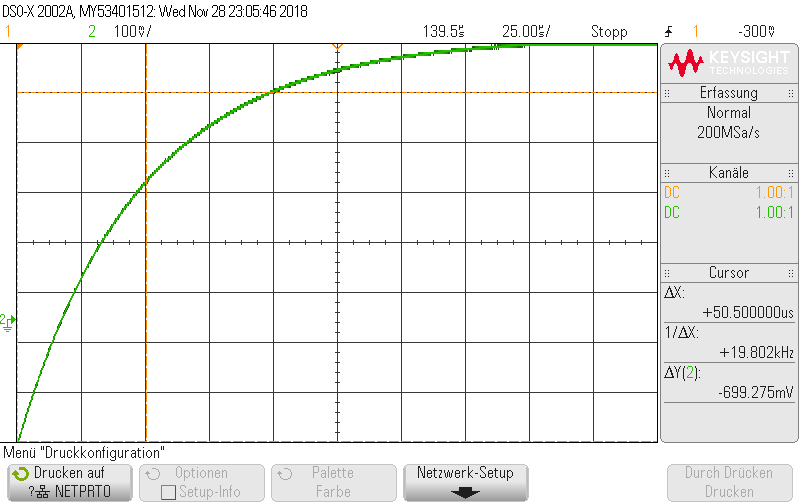
\includegraphics[width=\textwidth]{./img/ch2/58_methode.png}
	\centering
	\caption{Einschwingvorgangs des LR-Strangs}
	\label{fig:rl_einschwing}
\end{figure} \noindent
Ein entsprechender Single-Shot ist in Abbildung \ref{fig:rl_einschwing} zu sehen. Mit der draus erhaltenen Zeitkonstante von $\tau = 50.5 \mu$s ergibt sich eine Induktivität von
\begin{equation}
	L = \tau R = \tau (R_L + R_i) = 50.5 \mu s (17.8 + 986.15) \Omega = 50,699\,\text{mH}
\end{equation}
\section{Leistungsmessung}
TODO \\
TODO \\
TODO \\
\begin{figure}[H]
	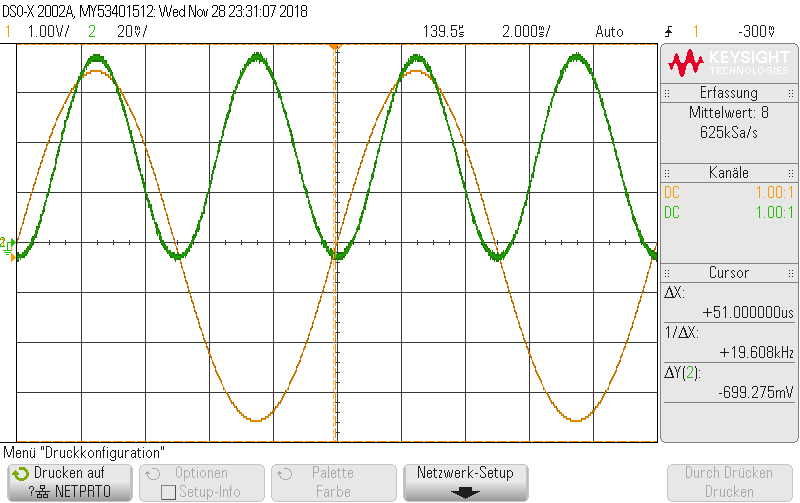
\includegraphics[width=\textwidth]{./img/ch2/leistung.png}
	\centering
	\label{XXXXX}
\end{figure}